% ------------------------------------------------------------------------
% MODELO ADAPTADO PARA GRADUAÇÃO EM SISTEMAS DE INFORMAÇÃO - UNIMONTES
% ESTRUTURA MODULAR
% ------------------------------------------------------------------------

\documentclass[
    12pt,               
    openright,          
    oneside,            
    a4paper,            
    english,            
    french,             
    spanish,            
    brazil              
    ]{unimontes-si-abntex2}
    
% ---
% Pacotes para Desenhos e Autômatos
% ---
\usepackage{tikz}
\usetikzlibrary{automata, positioning, arrows.meta}

% ---
% Pacotes básicos 
% ---
\usepackage{subcaption}
\usepackage{amsmath} 
\usepackage{amsfonts}
\usepackage{amssymb}
\usepackage{mathptmx} % Fonte Times New Roman exigida pela Unimontes    
\usepackage[T1]{fontenc}        
\usepackage[utf8]{inputenc}     
\usepackage{lastpage}           
\usepackage{indentfirst}        
\usepackage{color}              
\usepackage{graphicx}           
\usepackage{microtype}
\usepackage{longtable}
\usepackage{multirow}
\usepackage{array}
\usepackage{tabularx}
\usepackage{booktabs}
\usepackage{caption}
\captionsetup{justification=raggedright, singlelinecheck=false} % legendas e fontes alinhadas à esquerda (ABNT)
\AtBeginDocument{\renewcommand{\configurecaptions}{\captionsetup{justification=raggedright, singlelinecheck=false}}} % idem para tabelas em \IBGEtab
\usepackage{chngcntr}
\usepackage{float}


\usepackage{listings}
\usepackage{xcolor}

% Definição de cores
\definecolor{codegreen}{rgb}{0.2,0.8,0.2}
\definecolor{codegray}{rgb}{0.7,0.7,0.7}
\definecolor{codepurple}{rgb}{0.7,0.3,0.9}
\definecolor{codeviolet}{rgb}{0.6,0.2,0.9}

% Configuração global do lstlisting (padrão ABNT)
\lstset{
    language=SQL,
    backgroundcolor=\color{white},
    basicstyle=\ttfamily\small\color{black},
    keywordstyle=\color{codeviolet},
    commentstyle=\color{codegreen},
    stringstyle=\color{codepurple},
    numbers=left,
    numberstyle=\tiny\color{black},
    breaklines=true,
    showstringspaces=false,
    tabsize=2,
    frame=single,
    rulecolor=\color{black},
    captionpos=t,
    abovecaptionskip=3mm,      % Espaço acima do título (ABNT)
    belowcaptionskip=3mm,      % Espaço abaixo do título
    belowskip=4mm,             % Espaço após o código
    aboveskip=4mm              % Espaço antes do código
}

% ---
% Pacotes de Algoritmos (CONFIGURADOS PARA PORTUGUÊS)
% ---
\usepackage[ruled,linesnumbered,portuguese,onelanguage]{algorithm2e}

% Tradução manual dos títulos e legendas
\renewcommand{\listalgorithmcfname}{Lista de Algoritmos}
\renewcommand{\algorithmcfname}{Algoritmo}
\SetKwInput{KwIn}{Entrada}
\SetKwInput{KwOut}{Saída}

% Forçando as palavras-chave para Português (Padrão Teórico)
\SetKwFor{While}{enquanto}{faça}{fim}
\SetKwFor{For}{para}{faça}{fim}
\SetKwFor{ForEach}{para cada}{faça}{fim}
\SetKwIF{If}{ElseIf}{Else}{se}{então}{senão se}{senão}{fim}
\SetKw{Return}{retorne}

% Ajusta o contador para não zerar por capítulo
\AtBeginDocument{
    \counterwithout{algocf}{chapter}
    \counterwithout{lstlisting}{chapter}
}

% ---
% Pacotes de citações
% ---
\usepackage[alf]{abntex2cite}   % Citações padrão ABNT (Nominais)
\renewcommand{\ABNTEXchapterfont}{\rmfamily\bfseries}
\renewcommand{\ABNTEXsectionfont}{\rmfamily\bfseries}
\renewcommand{\ABNTEXsubsectionfont}{\rmfamily\bfseries}
\renewcommand{\ABNTEXsubsubsectionfont}{\rmfamily\bfseries}

% Importa o arquivo de configurações e comandos auxiliares (se houver)
% \input{configuracoes.tex} 

% ---
% Informações de dados para CAPA e FOLHA DE ROSTO
% ---
\titulo{Título do Trabalho de Conclusão de Curso}
\autor{Nome do(a) Autor(a)}
\local{Montes Claros - MG}
\data{Mês/Ano}
\orientador{Prof(a). Dr(a). Nome do(a) Orientador(a)}

\instituicao{
  Universidade Estadual de Montes Claros -- Unimontes
  \par
  Centro de Ciências Exatas e Tecnológicas -- CCET
  \par
  Curso de Bacharelado em Sistemas de Informação
}

\tipotrabalho{Projeto de Trabalho de Conclusão de Curso (Graduação)}

\preambulo{Projeto de Trabalho de Conclusão de Curso apresentado ao Curso de Sistemas de Informação da Universidade Estadual de Montes Claros, como requisito parcial para a obtenção do título de Bacharel em Sistemas de Informação.}

% ---
% Configurações de aparência do PDF final
\definecolor{blue}{RGB}{41,5,195}

\makeatletter
\hypersetup{
        pdftitle={\@title}, 
        pdfauthor={\@author},
        pdfsubject={\imprimirpreambulo},
        pdfcreator={LaTeX with abnTeX2},
        pdfkeywords={unimontes}{sistemas de informação}{tcc},
        colorlinks=true,               
        linkcolor=black, % Recomenda-se preto para impressão final             
        citecolor=black,                
        filecolor=black,              
        urlcolor=black,
        bookmarksdepth=4
}
\makeatother

% --- 
% Espaçamentos entre linhas e parágrafos exigidos pela Unimontes
% --- 
\setlength{\parindent}{2.0cm} % Recuo obrigatório de 2.0cm
\setlength{\parskip}{0.0cm}   % Sem espaçamento extra entre parágrafos

\makeindex

% ----
% Início do documento
% ----
\begin{document}

\selectlanguage{brazil}
\frenchspacing

% Ativa a adequação à NBR 10520:2023 (autor em caixa normal nas citações
% parentéticas e "et al." em itálico). Precisa ser a primeira citação processada.
\citeoption{abnt-opcoes-nbr2023}

% ----------------------------------------------------------
% ELEMENTOS PRÉ-TEXTUAIS
% ----------------------------------------------------------
\imprimircapa
\imprimirfolhaderosto*

% --- Ficha Catalográfica APENAS EM TCC
% \begin{fichacatalografica}
%     \sffamily
%     \vspace*{\fill}
%     \begin{center}
%     \fbox{\begin{minipage}[c][8cm]{13.5cm}
%     \small
%     \imprimirautor
%
%     \hspace{0.5cm} \imprimirtitulo  / \imprimirautor. --
%     \imprimirlocal, \imprimirdata.
%
%     \hspace{0.5cm} \pageref{LastPage} p. : il. (algumas color.) ; 30 cm.\\
%
%     \hspace{0.5cm} \imprimirorientadorRotulo~\imprimirorientador\\
%
%     \hspace{0.5cm}
%     \begin{minipage}{12cm}
%         \setlength{\parindent}{0pt}
%         \imprimirtipotrabalho~--~\imprimirinstituicao, \imprimirdata.
%     \end{minipage}\\
%
%     \hspace{0.5cm}
%         1. Palavra-chave 1.
%         2. Palavra-chave 2.
%         3. Palavra-chave 3.
%         I. \imprimirorientador.
%         II. Universidade Estadual de Montes Claros.
%     \end{minipage}}
%     \end{center}
% \end{fichacatalografica}


% --- Folha de aprovação APENAS EM TCC
%
%\begin{folhadeaprovacao}
%\begin{center}
%    {\ABNTEXchapterfont\large\textbf{{\imprimirautor}}}
%    \vspace*{\fill}\vspace*{\fill}
%    \begin{center}
%      \ABNTEXchapterfont\bfseries\Large{\imprimirtitulo}
%    \end{center}
%    \vspace*{\fill}
%    \hspace{.45\textwidth}
%    \begin{minipage}{.5\textwidth}
%        \imprimirpreambulo
%    \end{minipage}%
%    \vspace*{\fill}
%   \end{center}
%
%   Trabalho aprovado em: \_\_ de \_\_\_\_\_\_\_\_\_\_ de \_\_\_\_\_
%
%   \begin{center}
%     \vspace*{0.5cm}
%     \rule{10cm}{1pt} \\
%     \imprimirorientador \ (Orientador) -- Unimontes
%     \vspace*{0.5cm}
%     
%     \rule{10cm}{1pt} \\
%     Examinador 1 -- Unimontes
%     \vspace*{0.5cm}
%     
%     \rule{10cm}{1pt} \\
%     Examinador 2 -- Unimontes
%   \end{center}
%\end{folhadeaprovacao}

% --- Resumo na língua vernácula
% \setlength{\absparsep}{18pt}
% \begin{resumo}

 Texto do resumo em português, em parágrafo único e conciso, apresentando o tema, o problema de pesquisa, o objetivo geral, a metodologia empregada e o resultado esperado do trabalho. Recomenda-se entre 150 e 500 palavras, conforme a NBR 6028.

 \vspace{\onelineskip}
 \noindent \textbf{Palavras-chave}: Palavra-chave 1. Palavra-chave 2. Palavra-chave 3.
\end{resumo}


% --- Abstract
% % --- Abstract
\begin{resumo}[Abstract]
 \begin{otherlanguage*}{english}

Abstract text in English, as a single, concise paragraph, presenting the theme, the research problem, the general objective, the methodology used, and the expected outcome of the work.

\vspace{\onelineskip}
\noindent \textbf{Keywords}: Keyword 1. Keyword 2. Keyword 3.

 \end{otherlanguage*}
\end{resumo}


% --- Listas
\pdfbookmark[0]{\listfigurename}{lof}
\listoffigures*
\cleardoublepage

% Lista de Algoritmos
% \pdfbookmark[0]{\listalgorithmcfname}{loa}
% \listofalgorithms
% \cleardoublepage

% Lista de Tabelas
% \pdfbookmark[0]{\listtablename}{lot}
% \listoftables*
% \cleardoublepage

% Lista de Listagens
% \pdfbookmark[0]{\lstlistlistingname}{lol}
% \lstlistoflistings
% \cleardoublepage

% --- Lista de Listagens alterando o nome do inglês para português
\renewcommand{\lstlistlistingname}{Lista de Listagens}
\renewcommand{\lstlistingname}{Listagem}

% --- SUMÁRIO ---
\pdfbookmark[0]{\contentsname}{toc}
\tableofcontents*
\cleardoublepage
% -------------------------------------

% ----------------------------------------------------------
% ELEMENTOS TEXTUAIS
% ----------------------------------------------------------
\textual

% --- Chamando os capítulos modularizados ---
\chapter{Introdução}

Apresente aqui o contexto geral do trabalho: a área de conhecimento em que a pesquisa se insere, os fatos e conceitos que motivam o estudo, e um panorama de como o tema vem sendo tratado. Utilize citações de autores para embasar as afirmações apresentadas \cite{marconi2017metodologia}.

Em seguida, situe o leitor sobre o recorte específico do trabalho: o que exatamente será estudado, investigado ou desenvolvido, e sob qual abordagem (por exemplo, um estudo de caso, uma pesquisa experimental, uma revisão sistemática).

Por fim, descreva brevemente como o trabalho está estruturado, indicando o conteúdo de cada capítulo. Por exemplo:

Este trabalho está organizado em sete capítulos. O Capítulo 2 apresenta o tema e o problema de pesquisa, definindo a questão central a ser investigada. O Capítulo 3 apresenta os objetivos geral e específicos do trabalho. O Capítulo 4 expõe a justificativa da pesquisa, destacando sua relevância. O Capítulo 5 apresenta a fundamentação teórica, abordando os principais conceitos, tecnologias e trabalhos relacionados ao tema. O Capítulo 6 descreve as etapas metodológicas adotadas na pesquisa. Por fim, o Capítulo 7 apresenta o cronograma de execução das atividades previstas.

\chapter{Tema e Problema}

\section{Tema}

Descreva aqui o tema do trabalho em uma frase direta e objetiva, delimitando o assunto, o recorte metodológico e o contexto de aplicação da pesquisa. O tema costuma ficar bem alinhado ao próprio título do trabalho.

\section{Problema}

Descreva o problema de pesquisa: qual dificuldade, lacuna ou limitação prática motiva este trabalho? Explique as causas e consequências desse problema, e por que ele merece ser investigado.

Se houver um aspecto técnico ou prático que restrinja a pesquisa (por exemplo, limitações de tempo, de infraestrutura, de dados disponíveis), explicite-o aqui também.

Diante desse cenário, este trabalho busca responder à seguinte questão de pesquisa: [insira aqui a pergunta de pesquisa central, de forma clara e objetiva].

\chapter{Objetivos}
\label{sec:objetivos}

Este capítulo apresenta os objetivos que orientam o desenvolvimento da pesquisa.

\section{Objetivo Geral}

O objetivo geral deste trabalho é [verbo no infinitivo -- por exemplo: analisar, desenvolver, propor, comparar] [o que será feito], por meio de [abordagem/metodologia empregada], considerando [principais variáveis ou aspectos avaliados]\footnote{Exemplo de nota de rodapé com referência a um site: Disponível em: \url{https://www.exemplo.com/}. Acesso em: DD mês. AAAA.}.

\section{Objetivos Específicos}

OBS: Não confunda objetivo específico com metodologia de trabalho, isso é bastante comum.

Os objetivos específicos deste trabalho são:

\begin{itemize}[leftmargin=*,itemsep=0.5em]

\item Primeiro objetivo específico, geralmente relacionado à etapa inicial ou preparatória da pesquisa (ex.: levantar, revisar, implementar);

\item Segundo objetivo específico, relacionado à execução central da pesquisa (ex.: comparar, avaliar, aplicar);

\item Terceiro objetivo específico, relacionado à análise dos dados obtidos (ex.: analisar o impacto de determinada variável sobre os resultados);

\item Quarto objetivo específico, relacionado à conclusão ou síntese dos resultados (ex.: identificar a solução mais adequada segundo os critérios definidos).

\end{itemize}

\chapter{Justificativa}

Apresente aqui a relevância do tema escolhido: por que ele é importante, para quem, e que lacuna ou necessidade prática ou teórica ele atende. Utilize citações para embasar a relevância do tema com base na literatura \cite{marconi2017metodologia}.

Em seguida, aponte estudos recentes relacionados ao tema, destacando como eles reforçam a importância da pesquisa proposta. Por exemplo: \citeonline{marconi2017metodologia} destacam a importância de [aspecto relevante da literatura], o que sustenta o interesse em [conexão com o seu trabalho].

Por fim, explique a contribuição esperada do trabalho: o que se espera que os resultados tragam de benefício prático, acadêmico ou tecnológico para a área.

\chapter{Fundamentação Teórica}
\label{cap:FundamentacaoTeorica}

Este capítulo apresenta a fundamentação teórica necessária ao desenvolvimento da pesquisa, abordando os principais conceitos, técnicas e tecnologias relacionados ao tema. Cada seção deve corresponder a um conceito central para a compreensão da metodologia proposta -- evite incluir conceitos que não serão retomados na metodologia ou nos resultados.

\section{Nome do Primeiro Conceito}

Apresente aqui o primeiro conceito teórico relevante para o trabalho. Utilize citações para embasar as definições apresentadas. Há duas formas principais de citar um autor conforme a ABNT:

Na forma narrativa, o nome do autor faz parte da frase: \citeonline{marconi2017metodologia} definem o método científico como um conjunto de procedimentos sistemáticos para a produção de conhecimento válido.

Na forma parentética, a citação aparece entre parênteses ao final da frase, sem fazer parte da sintaxe da oração \cite{marconi2017metodologia}.

Para citar uma página específica de uma obra (recomendado em citações diretas), utiliza-se \citeonline[p.~10]{marconi2017metodologia}.

A Figura \ref{fig:exemplo} ilustra um exemplo de diagrama simples, construído diretamente em \LaTeX{};

\begin{figure}[H]
    \centering
    \caption{Exemplo de diagrama simples}
    \label{fig:exemplo}
    \centering
    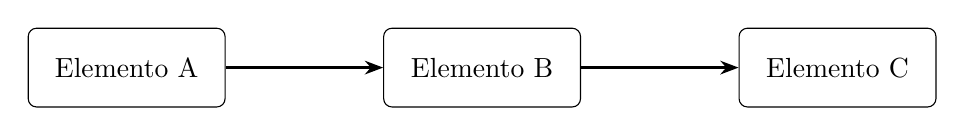
\begin{tikzpicture}[
        node distance=2cm, 
        every node/.style={draw, rectangle, minimum width=2.5cm, minimum height=1cm, align=center, rounded corners=3pt},
        >=Stealth
    ]
        \node (a) {Elemento A};
        \node (b) [right=of a] {Elemento B};
        \node (c) [right=of b] {Elemento C};
        
        \draw[->, thick] (a) -- (b);
        \draw[->, thick] (b) -- (c);
    \end{tikzpicture}
    \fonte{Elaborado pelo autor, 2026.}
\end{figure}

\section{Nome do Segundo Conceito}

Apresente aqui o segundo conceito teórico, por exemplo um algoritmo relevante para o trabalho. O Algoritmo \ref{alg:exemplo} ilustra o uso do pacote \textit{algorithm2e} (já configurado em português no preâmbulo) para descrever pseudocódigo.

OBS: Se citar figura ou algoritmo, tem que informar a página do livro ao qual referenciou na fonte da imagem ou algoritmo. ex:

\begin{algorithm}[H]
    \caption{Nome do algoritmo de exemplo}
    \label{alg:exemplo}
    \KwIn{$n$: um valor de entrada}
    \KwOut{$r$: o resultado calculado}
    $r \gets 1$\;
    \For{$i \gets 1$ \KwTo $n$}{
        $r \gets r \times i$\;
    }
    \Return{$r$}\;
\end{algorithm}
\fonte{\citeonline[p.~XX]{marconi2017metodologia}. Substitua pela referência e página reais do livro de onde o algoritmo foi adaptado.}

\section{Nome do Terceiro Conceito}

Se o trabalho envolver algum tipo de código-fonte (consultas, scripts, trechos de configuração), utilize \verb|\lstinputlisting| para importar o código de um arquivo externo, mantendo-o destacado do texto corrido e numerado como Listagem. A Listagem \ref{lst:exemplo} apresenta um exemplo.

\lstinputlisting[
    language=SQL,
    caption={Exemplo de criação de tabela},
    label={lst:exemplo}
]{sql/department.sql}
\vspace{-0.4cm}
\fonte{\citeonline[p.~14]{silberschatz2020database}.}

\section{Trabalhos Relacionados}

Encerre a fundamentação teórica com uma seção que situe o trabalho perante a literatura já existente sobre o tema. Para cada trabalho relacionado relevante, apresente: (i) o que o autor fez; (ii) qual metodologia ou abordagem foi utilizada; (iii) quais os principais resultados; e (iv) como esse trabalho se relaciona com a pesquisa proposta.

Por exemplo: \citeonline{marconi2017metodologia} discutem [aspecto relevante], utilizando [metodologia/abordagem], concluindo que [principal resultado]. Esse achado é relevante para este trabalho pois [conexão direta com a pesquisa proposta].

Ao final da seção, é recomendável indicar explicitamente a lacuna identificada na literatura que este trabalho pretende preencher, deixando claro o ineditismo ou a contribuição da pesquisa.

\chapter{Procedimentos Metodológicos}
\label{cap:metodologia2x}

Apresente aqui uma visão geral do objeto de estudo (base de dados, sistema, população, amostra etc.) e do contexto em que a pesquisa será conduzida. Não podemos deixar entre capítulos e seções, espaço em branco e sem texto, como seria se não existisse esse parágrafo atual, isos vale para o documento todo.

\section{Caracterização da Pesquisa}
\label{sec:caracterizacao}

Classifique a pesquisa quanto às quatro dimensões metodológicas mais comuns, sempre justificando o enquadramento escolhido:

Quanto à natureza, classifique como básica ou aplicada. Quanto à abordagem do problema, classifique como quantitativa, qualitativa ou quali-quantitativa. Quanto aos objetivos, classifique como exploratória, descritiva ou explicativa. Quanto aos procedimentos técnicos, classifique como bibliográfica, documental, experimental, estudo de caso, entre outros \cite{marconi2017metodologia}. Use uma boa referência de livro de metodologia.

\section{Etapas da Pesquisa}

Descreva as macroetapas que estruturam a pesquisa do início ao fim (por exemplo: preparação, definição de variáveis, execução/coleta e análise), explicando brevemente o que ocorre em cada uma antes de detalhá-las em subseções.

\subsection{Etapa 1 -- Nome da Primeira Etapa}

Descreva a primeira etapa da pesquisa (por exemplo: preparação do ambiente, da base de dados ou do material que será utilizado).

\subsection{Etapa 2 -- Definição das Variáveis e do Plano de Testes}

Caso a pesquisa seja experimental, defina aqui a variável de controle (o que será mantido fixo para não interferir na análise), a variável independente (o que será manipulado) e a variável dependente (o que será medido como resultado) \cite{marconi2017metodologia}.

A Tabela \ref{tab:plano_testes} apresenta um exemplo de plano de testes, combinando as variáveis independentes definidas para compor os cenários experimentais.

\begin{table}[H]
\IBGEtab{
\caption{Plano de testes experimental}
\label{tab:plano_testes}
}{
\begin{tabular}{c c c c}
\hline
\textbf{Caso} &
\textbf{Variável A} &
\textbf{Variável B} &
\textbf{Métricas Coletadas} \\
\hline

C1 & Valor 1 & Valor 1 & Métrica 1, Métrica 2 \\
C2 & Valor 1 & Valor 2 & Métrica 1, Métrica 2 \\
C3 & Valor 2 & Valor 1 & Métrica 1, Métrica 2 \\
C4 & Valor 2 & Valor 2 & Métrica 1, Métrica 2 \\

\hline
\end{tabular}
}{
\vspace{0.3cm}
\fonte{Elaborado pelo autor, 2026.}
}
\end{table}

\subsection{Etapa 3 -- Execução e Coleta das Métricas}

Descreva como os experimentos (ou a coleta de dados) serão executados na prática, e com quais ferramentas as métricas de interesse serão obtidas.

\subsection{Etapa 4 -- Análise dos Resultados}

Descreva como os dados coletados serão analisados (por exemplo: estatística descritiva, comparação entre cenários, testes de hipótese) e como essa análise responderá à questão de pesquisa apresentada no Capítulo 2.

\chapter{Cronograma}
\label{cap:cronograma}

O cronograma de atividades para o desenvolvimento deste trabalho é apresentado na Tabela \ref{tab:cronograma}, considerando um período de execução de 11 meses. O planejamento contempla as etapas metodológicas definidas neste projeto, além da fundamentação teórica e da redação final da monografia.

As atividades previstas no cronograma são:

\begin{enumerate}
    \item Redação da monografia;
    \item Etapa 1 -- Nome da primeira etapa;
    \item Etapa 2 -- Nome da segunda etapa;
    \item Etapa 3 -- Nome da terceira etapa;
    \item Etapa 4 -- Nome da quarta etapa;
    \item Ajustes finais e defesa do TCC.
\end{enumerate}

\begin{table}[htb]
\IBGEtab{
\caption{Cronograma de atividades para o desenvolvimento do TCC.}
\label{tab:cronograma}
}{
\footnotesize
\begin{tabularx}{\textwidth}{>{\raggedright\arraybackslash}X*{11}{c}}
\toprule
\textbf{Atividades} & \textbf{M1} & \textbf{M2} & \textbf{M3} & \textbf{M4} & \textbf{M5} & \textbf{M6} & \textbf{M7} & \textbf{M8} & \textbf{M9} & \textbf{M10} & \textbf{M11} \\
\midrule
1 & X & X & X & X & X & X & X & X & X & X & X \\
2 & & X & X & X & & & & & & & \\
3 & & & X & X & X & X & & & & & \\
4 & & & & X & X & X & X & X & X & & \\
5 & & & & & & & & X & X & X & \\
6 & & & & & & & & & & X & X \\
\bottomrule
\end{tabularx}
}{
\vspace{0.3cm}
\fonte{Elaborado pelo autor, 2026.}
}
\end{table}

As atividades foram organizadas de forma a permitir o desenvolvimento progressivo das etapas metodológicas propostas, garantindo tempo adequado para a fundamentação teórica, a execução da pesquisa, a análise dos resultados e a redação final da monografia.


% ----------------------------------------------------------
% ELEMENTOS PÓS-TEXTUAIS
% ----------------------------------------------------------
\postextual

\bibliography{abntex2-modelo-references} 

% --- Apêndices

% \begin{apendicesenv}
% \partapendices
% \end{apendicesenv}
% \begin{anexosenv}
% \partanexos
% \end{anexosenv}

\end{document}
